\documentclass[tikz,border=5pt]{standalone}
\usepackage{tikz}
\usetikzlibrary{arrows.meta,positioning,calc}
\definecolor{nebula}{HTML}{6366F1}
\definecolor{spark}{HTML}{14B8A6}
\definecolor{ink}{HTML}{334155}
\begin{document}
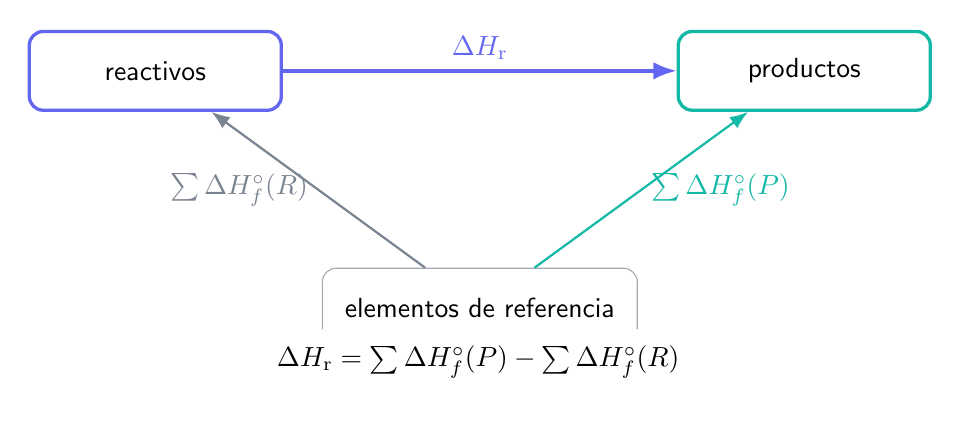
\begin{tikzpicture}[font=\sffamily,>=Latex,node distance=2.7cm]
  \node[draw=nebula,very thick,rounded corners=5pt,minimum width=3.2cm,minimum height=1cm] (r) {reactivos};
  \node[draw=spark,very thick,rounded corners=5pt,minimum width=3.2cm,minimum height=1cm,right=5cm of r] (p) {productos};
  \node[draw=ink!45,rounded corners=5pt,minimum width=4cm,minimum height=1cm,below=2.5cm of $(r)!0.5!(p)$] (e) {elementos de referencia};
  \draw[->,very thick,nebula] (r)--(p) node[midway,above] {$\Delta H_{\rm r}$};
  \draw[->,thick,ink!65] (e)--(r) node[midway,left] {$\sum\Delta H_f^\circ(R)$};
  \draw[->,thick,spark] (e)--(p) node[midway,right] {$\sum\Delta H_f^\circ(P)$};
  \node[fill=white,rounded corners=4pt,inner sep=6pt] at (4.1,-3.7) {$\Delta H_{\rm r}=\sum\Delta H_f^\circ(P)-\sum\Delta H_f^\circ(R)$};
\end{tikzpicture}
\end{document}
